\chapter{Introduction}
%Este manual tem como objetivo mostrar o uso das ferramentas
%do InVesalius e também apresentar alguns conceitos para facilitar
%a utilização do software.

This manual aims to show the use of InVesalius tools and also present some concepts to facilitate the use of the software.

%O InVesalius é um software para auxiliar o profissional
%de saúde no diagnóstico	e no planejamento cirúrgico. Cabe
%ressaltar, porém, que todo software no contexto de diagnóstico é
%totalmente suplementar, pois todo e qualquer ato cometido é de
%inteira responsabilidade do profissional de saúde.

InVesalius is a software that is designed to assist health professionals on diagnosis and surgical planning. It should be noted, however, that all software in the diagnostic context is fully supplementary, and each and every act committed is the responsibility of health professionals.
 
%Além da medicina, é possível utilizar o software em outras áreas, como
%arqueologia, veterinária, ou mesmo em aplicações industriais.
%Como requisito básico, basta que as imagens a serem analisadas
%estejam no padrão DICOM (\textsl{Digital Imaging Communications in Medicine}).
%Até o presente momento, o InVesalius reconstrói
%imagens provindas de tomógrafos e de aparelhos de ressonância magnética.
%Para operar o software, basta ter conhecimentos básicos de 
%informática. Noções básicas sobre imagens médicas podem contribuir para o
%melhor entendimento das operações.

In addition to the medicine, you can use the software in other areas such as archaeology, medicine, dentistry, veterinary, or even in industrial applications. As a basic requirement, the images to be analyzed are in DICOM (Digital Imaging Communications in Medicine). To date, InVesalius reconstructs images stemmed from CT scanners and MRI machines. To operate the software, one needs to posses basic computer skills cos. Understanding medical images can help to form a better understanding of the operations.

%\section{Conceitos importantes}
\section{Important Concepts}

%Nesta seção, discutiremos alguns conceitos necessários para melhor
%entendimento e operação do software.
In this section, we discuss some concepts necessary to better understanding of and operation of the software.

\subsection{DICOM (\textit{Digital Image Communications in Medicine})}			
%DICOM é um padrão relativo à transmissão, ao armazenamento e
%ao tratamento de imagens médicas. O padrão prevê diversas modalidades de imagens médicas,
%como imagens provindas de equipamentos de tomografia computadorizada, ressonância magnética,
%ultrassom, eletrocardiograma, entre outras.

DICOM is a standard on the transmission, storage and treatment of medical images. The standard provides various types of medical images, such as images emanating from computed tomography equipment, magnetic resonance, ultrasound, electrocardiogram, among others.

%Uma imagem DICOM é composta por 2 itens principais, uma matriz contendo os pixels da
%imagem e um conjunto de meta-informações. Essas informações contêm, por exemplo, o nome
%do paciente, a modalidade da imagem e a posição da imagem em relação ao espaço (no caso
%de tomografia e ressonância).

A DICOM image consists of two main components, namely, an array containing the pixels of the image and a set of meta-information. This information includes, but is not limited to, patient name, mode image and the image position in relation to the space (in the case of CT and MRI).

\subsection{Computed Tomography - Medical}
%A tomografia computadorizada indica a radiodensidade dos tecidos, isto é, a média de
%absorção de raios-X pelos tecidos. A radiodensiade é traduzida para a imagem em níveis
%de cinza em uma escala chamada \textit{Hounsfield}, nome dado em homenagem a Godfrey
%Newbold Hounsfield, um dos criadores da primeira máquina de tomografia computadorizada.

Computed tomography indicates the radiodensity of tissues, i.e., the average X-ray absorption by the tissues. The radiodensiade is translated into an image in gray levels, called the \textit{Hounsfield} scale, named after Godfrey Newbold Hounsfield, one of the creators of the first CT scan machine.

\begin{figure}[!htb]
\centering
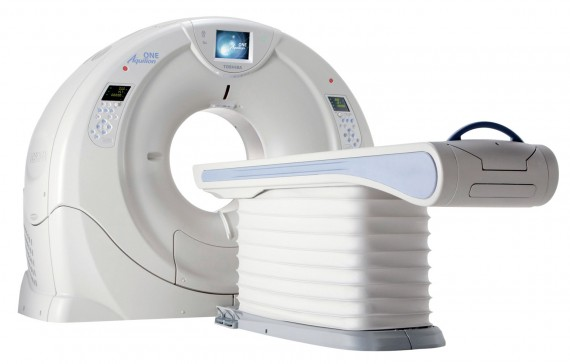
\includegraphics[scale=0.4]{tomografo.jpg}
\caption{Medical CT scanner - www.toshibamedical.com.br}
\end{figure}

%Nos aparelhos mais modernos, com um emissor de radiação e um banco de
%sensores (também chamados de canais, variando de 2 até 256), que circundam o paciente
%enquanto a maca é movimentada, formando uma espiral, é possível gerar uma
%grande quantidade de imagens, simultaneamente, com pouca emissão de raios-X.

In the most modern appliances, with a radiation emitter and a sensor bank (also called channels, ranging from 2 to 256), which circumvent the patient while the stretcher is moved, forming a spiral, it is possible to generate a large number of images simultaneously, with little emission of X-rays.

%\subsubsection{Escala de Hounsfield}
\subsubsection{Hounsfield Scale}

%Como citado na seção anterior, as imagens de tomografia computadorizada
%são geradas em níveis de cinza, os quais são depois traduzidos na escala
%de Hounsfield (HU). Os tons mais claros representam tecidos mais densos, e
%os mais escuros, tecidos menos densos, como a pele e o cérebro.
As mentioned in the previous section, the CT images are generated in gray levels, which are then translated in the range of Hounsfield (HU). The lighter shades represent denser fabrics, and the darker, less dense tissue such as skin and brain. 

%A tabela \ref{tab:escala_hounsfield} apresenta alguns materiais e seus 
%respectivos valores em HU (\textit{Hounsfield Unit}).

Table~\ref{tab:escala_hounsfield} presents some materials and their repective values in HU (\textit{Hounsfield Unit}).

\begin{table}[h]
\centering
\caption{Escala de Hounsfield}
\begin{tabular}{lcc}\\
\hline % este comando coloca uma linha na tabela
Material & HU\\
\hline
\hline
Air & -1000 or less\\
Fat & -120\\
Water & 0\\
Muscle & 40\\
Contrast & 130\\
Bone & 400 or more\\
\hline
\end{tabular}
\label{tab:escala_hounsfield}
\end{table}


\subsection{Computed Tomography - Dental (CBCT)}

%A tomografia computadorizada odontológica comumente trabalha com menos emissão
%de radiação se comparada à tomografia computadorizada médica e, em consequência,
%torna possível visualizar mais detalhes de regiões delicadas, como a cortical alveolar.

The dental CT commonly works with less radiation emission if compared to medical CT, and therefore makes it possible to view more details of delicate regions such as alveolar cortical.

\begin{figure}[!htb]
\centering
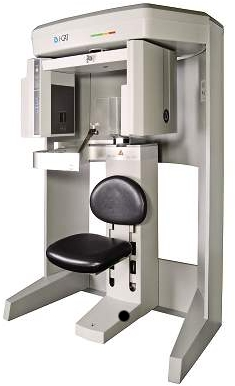
\includegraphics[scale=0.4]{feixe_conico.jpg}
\caption{Detal tomography - www.kavo.com.br}
\end{figure}

%A aquisição das imagens é feita com o paciente na vertical (ao contrário da tomografia médica,
%em que o paciente fica na horizontal). Um emissor e um sensor de raios-X circundam o crânio
%do paciente, formando um arco de $180^\circ$ ou $360^\circ$. As imagens geradas pelo tomógrafo
%podem ser interpretadas como um volume com o crânio do paciente imerso. Esse volume é "fatiado"
%pelo software do aparelho, podendo-se gerar imagens com espaçamentos diferentes ou outros
%tipos de imagens, como a visão panorâmica da região de interesse.

Image acquisition is performed with the patient in the vertical (as opposed to medical tomography, the patient is horizontal). A transmitter and a sensor X-ray surround the patient's skull, forming an arc of $180^\circ$ or $360^\circ$. The images generated by the scanner can be interpreted as a volume with the skull immersed patient. This volume is "sliced" by the instrument software, being able to generate images with different spacing or other types of images, such as the panoramic view of the region of interest.

%As imagens adquiridas por tomógrafos odontológicos costumam exigir um maior pós-processamento
%quando é necessário separar (segmentar) determinadas estruturas usando outros softwares como
%o InVesalius. Isso ocorre porque, normalmente, essas imagens possuem mais níveis de cinza que
%a escala de Hounsfield, o que torna o uso de padrões de segmentação \textit{(presets)} menos
%eficiente. Outra característica bastante comum nas imagens provindas de tomógrafos
%odontológicos é a alta presença de ruídos do tipo \textit{speckle} e a presença de outros
%ruídos normalmente causados por uso de próteses de amálgama pelo paciente.

The images acquired by dental scanners often require more post processing when it is necessary to separate (segmental) certain structures using other software such as InVesalius. This is because, typically, these images have more gray levels than the study shut Hounsfield, which makes the use of segmentation patterns (preset) less efficient. Another very common feature in the images of provincial dental CT scanners is the high presence of speckle noise type and the presence of other noise typically caused by the use of amalgam prosthesis by the patient.

\subsection{Magnetic Resonance Imaging - MRI}

%A ressonância magnética é um exame realizado sem o uso de radiação ionizante. Em vez disso,
%é utilizado um forte campo magnético para alinhar os átomos de algum elemento presente em
%nosso corpo, comumente o hidrogênio. Após o alinhamento, são disparadas ondas de rádio, e os
%átomos são excitados. Os sensores medem o tempo que os átomos de hidrogênio demoram para se
%alinhar novamente. Com isso, é possível determinar qual é o tipo de tecido, pois tecidos
%diferentes apresentam quantidades diferentes de átomos de hidrogênio.

MRI is an examination performed without the use of ionizing radiation. Instead, it used a strong magnetic field to align the atoms of any element present in our body, commonly the nio hydrogenated. After alignment, radio waves are triggered, and atoms are excited. The sensors measure the time that the hydrogen atoms democratic ram to align again. This makes it possible to determine what kind of fabric, because different tissues have different amounts of hydrogen atoms.

%Para evitar interferências e melhorar a qualidade do sinal de radiofrequência, além de o
%paciente ficar dentro do equipamento, é colocada uma bobina na região de interesse.

To avoid interference and improve the quality of the radiofrequency signal, and the patient get inside the machine, it is placed a coil in the region of interest.

\begin{figure}[!htb]
\centering
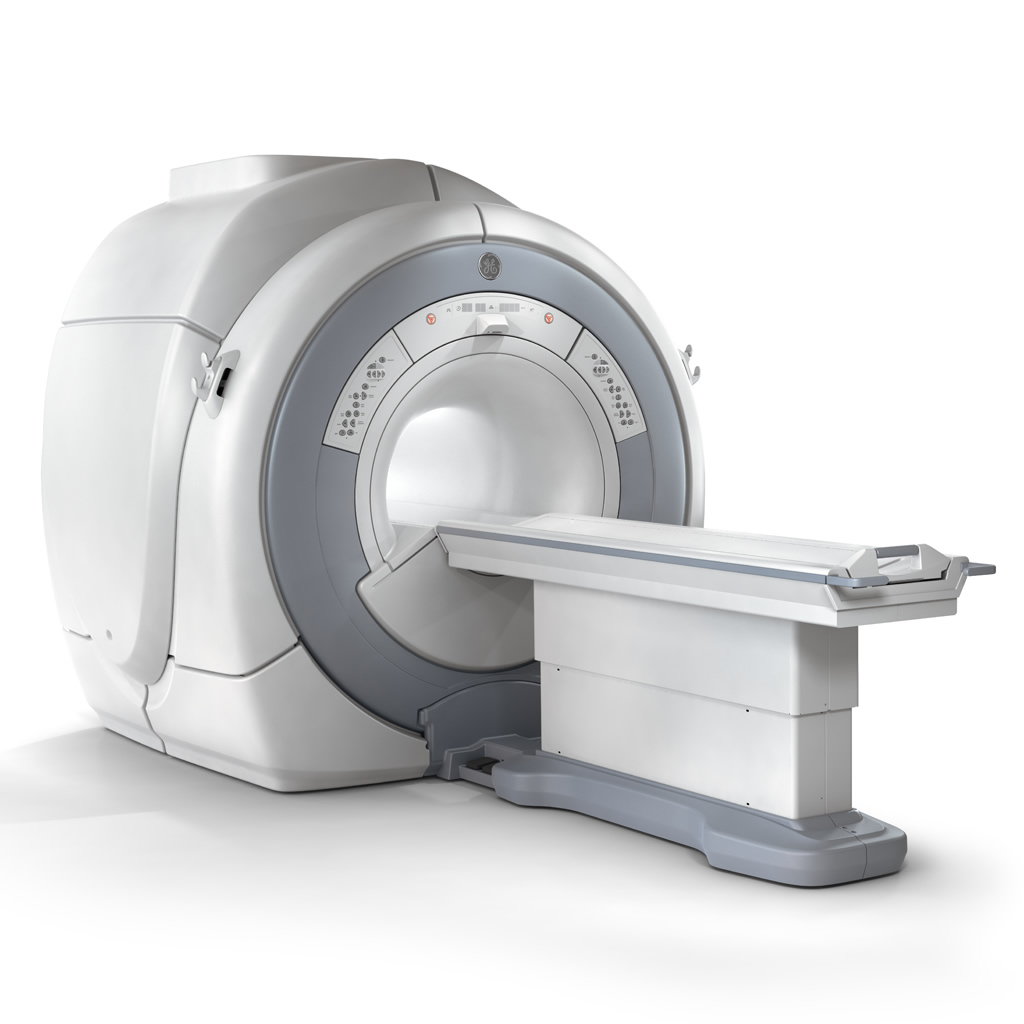
\includegraphics[scale=0.2]{rm_ge.jpg}
\caption{Magnetic resonance imaging equipment - www.gehealthcare.com}
\end{figure}

\begin{figure}[!htb]
\centering
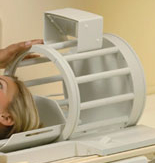
\includegraphics[scale=0.8]{bobina.jpg}
\caption{Coil - www.healthcare.philips.com}
\end{figure}

\subsection{Neuronavigation}
\label{sec:neuronavegador_intro}

Neuronavigation is a technique that allows tracking and localization of surgical instruments relative to neuronal
structures through computer visualization. In addition, neuronavigation systems have been pointed out as a fundamental
tool to aid surgical planinng and to increase the accuracy of experiments in neuroscience, such as transcranial magnetic
stimulation (TMS), electroencephalography (EEG), magnetoencephalography (MEG) and near-infrared spectroscopy (NIRS).
Despite the vast field of applications, the use of neuronavigation in research centers is limited by its high cost.
InVesalius Navigator offers users a low-cost, open-source alternative to commercial navigation systems. In this sense,
it is possible to use specific tools for neuronavigation and still have the possibility of developing features on demand.
The software for neuronavigation is distributed in an executable version compatible with Windows 7, 8 and 10 operating
system. The chapter~\ref{sec:neuronavegador} goes into details of all features of neuronavigation in InVesalius.


%\section{Recursos necessários}
\section{Resources needed}

%O InVesalius é projetado para executar em computadores pessoais, como
%\textit{desktops} e \textit{notebooks}. Atualmente, ele é compatível com
%os seguintes sistemas operacionais:\\
The InVesalius is designed to run on personal computers, such as desktops and notebooks. Currently, it is compatible with the following operating systems:\\
- MS-Windows (Windows 7, 8 e 10)\\
- GNU/Linux (Ubuntu, Mandriva, Fedora)\\
- Apple Mac OS X

%O desempenho do InVesalius depende, principalmente, da quantidade de fatias
%reconstruídas (imagens abertas pelo software), da quantidade de memória RAM
%disponível, da frequência do processador e da arquitetura do sistema operacional
%(32 \textit{bits} ou 64 \textit{bits}).

The performance of InVesalius depends mainly on the amount of reconstructed slices (images offered by the software), the amount of memory available RAM, the processor frequency and operating system architecture (32-bit or 64-bit).

%Vale ressaltar, como regra geral, que quanto maior a quantidade de memória RAM
%disponível no sistema, maior será o número de fatias que podem ser abertas
%simultaneamente para um dado estudo. Por exemplo, com 1 GB de memória disponível,
%pode-se abrir cerca de 300 fatias com resolução de 512x512 \textit{pixels}.
%Já com 4 GB de memória, pode-se abrir em torno de 1000 imagens com a mesma
%resolução.
It is noteworthy, as a general rule, the greater the amount of memory available RAM on the system, the greater the number of slices that can be opened simultaneously for a given study. For example, with 1 GB of available memory, it can open about 300 slices with a resolution of 512x512 pixels. Now with 4GB of memory, it can be opened around 1000 images at the same resolution.

			
%\subsection{Configurações mínimas}
\subsection{Minimum settings}
32 \textit{bits} Operating System\\
Intel Pentium 4 or equivalent with frequency 1,5 GHz\\
1 GB RAM\\
80 GB hard disk\\
Graphics card  with 64 MB de memória\\
Video resolution of 1024x768 \textit{pixels}


%\subsection{Configurações recomendadas}
\subsection{Recommended settings}
64 \textit{bits} Operating System\\
Intel Core 2 Duo processor or equivalent, with a frequency of 2.5 GHz\\
4GB of RAM\\
180 GB of hard disk\\
NVidia or ATI graphics card with 128 MB of memory\\
Video resolution of 1024x768 \textit{pixels}

